\documentclass[12pt,a4paper]{article}
\usepackage{amsmath}
\usepackage{amsfonts}
\usepackage{amssymb}
\usepackage{polski}
\usepackage{indentfirst}
\usepackage{graphicx}
\usepackage{natbib}
\usepackage{verbatim}
\usepackage{commath}
\usepackage{url}
\usepackage{hyperref}
\usepackage[margin=1in]{geometry}

\begin{document}

\title{Analiza i Przetwarzanie Dźwięku - Sprawozdanie z projektu 1.}
\author{Szymon Tomulewicz}
\date{9 IV 2020}
\maketitle
\tableofcontents
\newpage

\section{Wprowadzenie\label{sec:wprowadzenie}}
Celem projektu było stworzenie aplikacji okienkowej, umożliwiającej wczytywanie plików wav,
a następnie analizowanie ich pod kątem wybranych parametrów i wartości.

\subsection{Aplikacja\label{sec:aplikacja}}
Aplikacja została wykonana w języku C\#, przy użyciu biblioteki NAudio do przetwarzania i analizy
plików dźwiękowych, oraz biblioteki WinForms do stworzenia interfejsu oraz wyświetlania parametrów.
Wybrałem NAudio ze względu na popularność tej biblioteki, ilość dokumentacji oraz integrację z
biblioteką WinForms.

Aplikacja składa się z jednego widoku (Rys. \ref{fig:app}), na którym po załadowaniu pliku
dźwiękowego rysują się wykresy parametrów opisanych w dalszej części sprawozdania.

\begin{figure}[h!]
\centering
\includegraphics[width=1.0\textwidth]{figures/app}
\caption{Przykładowy stan aplikacji}
\label{fig:app}
\end{figure}

Użytkownik może podać w interfejsie dwie wartości: długość ramki w milisekundach oraz parametr (tzw.
\emph{lag}) używany w funkcji autokorelacji oraz AMDF (Average Magnitude Difference Function). Jako
jednostkę parametru \emph{lag} aplikacja przyjmuje liczbę próbek.

\section{Obliczane parametry\label{sec:parametry}}
Wszystkie obliczenia w aplikacji, które są wykonywane na próbkach, używają typów
zmiennoprzecinkowych. NAudio umożliwia to przy użyciu metody \verb|ToSampleProvider|:

\begin{verbatim}
    using (WaveFileReader reader = new WaveFileReader(filePath))
    {
        // Convert to 32-bit floating point samples:
        ISampleProvider sampleProvider = reader.ToSampleProvider();
        ...
        float[] buffer = new float[frameSizeFloats];
        ...
        sampleProvider.Read(buffer, 0, frameSizeFloats);
        ...
    }
\end{verbatim}

\subsection{Parametry w dziedzinie czasu na poziomie ramki (Frame-level)\label{sec:framelevel}}
Parametry opisane w kolejnych sekcjach są obliczane, a następnie zapisywane i wyświetlane w formie
wykresów (Rys. \ref{fig:app_preview}). $N$ występujące we wzorach oznacza zwykle długość ramki w
próbkach.

\subsubsection{STE - Short Time Energy\label{sec:ste}}
Dla n-tej ramki, $STE$ wynosi:
\begin{equation}
    STE(n)=\frac{1}{N}\sum_{i=0}^{N-1}s_n^2(i)
\end{equation}
Gdzie $s_n(i)$ to amplituda i-tej próbki w n-tej ramce.

\subsubsection{Volume - głośność\label{sec:volume}}
Dla n-tej ramki, głośność wynosi:
\begin{equation}
    v(n)=\sqrt{STE(n)}
\end{equation}

\subsubsection{ZCR - Zero Crossing Rate\label{sec:zcr}}
Dla n-tej ramki, $ZCR$ wynosi
\begin{equation}
    Z(n)=\frac{1}{N2}\bigg(
        \sum_{i=1}^{N-1} \abs{sign(s_n(i))-sign(s_n(i-1))}
    \bigg)
\end{equation}
Gdzie $sign$ to funkcja signum. Zrezygnowałem z mnożenia wyniku przez częstotliwość próbkowania,
ponieważ niepotrzebnie uzależniało to $ZCR$ od kolejnej wartości, a co za tym idzie utrudniało
określanie progów (np. \ref{sec:silent}).

\subsubsection{Częstotliwość tonu podstawowego\label{sec:f0}}
W nadziei na możliwość obliczenia tonu podstawowego zaimplementowałem obliczanie następujących
funkcji:
\begin{itemize}
\item
    Funkcji autokorelacji:
    \begin{equation}
        R_n(l)=\sum_{i=0}^{N-l-1}s_n(i)s_n(i+l)
    \end{equation}
\item
    Funkcji AMDF (Average Magnitude Difference Function):
    \begin{equation}
        A_n(l)=\sum_{i=0}^{N-l-1}\abs{s_n(i+l)-s_n(i)}
    \end{equation}
\end{itemize}
Gdzie $s_n(i)$ oznacza amplitudę i-tej próbki w n-tej ramce, a $l$ - parametr $lag$ podany przez
użytkownika.

Niestety dla tych parametrów, operacja obliczania (a właściwie przybliżania) częstotliwości tonu
podstawowego okazała się zbyt kosztowna (Zob. \cite{leszczyna}) na potrzeby tego projektu.

\subsection{Cechy sygnału audio na poziomie klipu (Clip-level)\label{sec:cliplevel}}
Parametry opisane w kolejnych sekcjach są obliczane, a następnie zapisywane i wyświetlane na dole
widoku (Rys. \ref{fig:app_preview}). Liczba ramek, na które został podzielony klip oznaczana jest
jako $F$.

\subsubsection{VSTD\label{sec:vstd}}
Odchylenie standardowe znormalizowane przez maksymalną wartość głośności w całym klipie.
\begin{equation}
    VSTD=\frac{1}{max(v)}\sqrt{
        \sum_{n=0}^{F-1}\big(
            v(s_n) - avg(v)
        \big)^2
    }
\end{equation}
Gdzie , $v(s_n)$ - głośnością w n-tej ramce, $max(v)$ - maksymalną wartością głośności w całym
klipie, a $avg(v)$ - średnią głośnością w całym klipie.

\subsubsection{ZSTD\label{sec:zstd}}
Analogicznie liczone jest odchylenie standardowe $ZCR$. W tym wypadku jednak aplikacja nie
normalizuje otrzymanej wartości.
\begin{equation}
    ZSTD=\sqrt{
        \sum_{n=0}^{F-1}\big(
            z(s_n) - avg(z)
        \big)^2
    }
\end{equation}
Gdzie $z(s_n)$ jest wartością $ZCR$ w n-tej ramce, a $avg(z)$ - średnią wartością $ZCR$ w całym
klipie.

\subsubsection{VDR - Volume dynamic range\label{sec:vdr}}
\begin{equation}
VDR=\frac{max(v)-min(v)}{max(v)}
\end{equation}
Gdzie $max(v)$ to maksymalna głośność w klipie, a $min(v)$ - minimalna.

\subsubsection{LSTER - Low Short Time Energy Ratio\label{sec:lster}}
\begin{equation}
    LSTER=\frac{1}{2F}\sum_{n=0}^{F-1}[
        sgn(0.5*avg(STE)-STE(n)+1
    ]
\end{equation}
Gdzie $avg(STE)$ to średnia wartość $STE$ w jednosekundowym oknie, a $STE(n)$ - wartość $STE$ w
n-tej ramce.

\subsubsection{HZCRR - High Zero Crossing Rate Ratio\label{sec:hzcrr}}
\begin{equation}
    HZCRR=\frac{1}{2F}\sum_{n=0}^{F-1}[
        sgn(ZCR(n)-1.5*avg(ZCR))+1
    ]
\end{equation}
Gdzie $avg(ZCR)$ to średnia wartość ZCR w jednosekundowym oknie, a $ZCR(n)$ - wartość $ZCR$ w n-tej
ramce.

\section{Metody\label{sec:metody}}
Po obliczeniu poprzednich wartości, aplikacja przechodzi do wykrywania ciszy oraz kategoryzowania
mowy.

\subsection{Wykrywanie ciszy\label{sec:silent}}
Aplikacja wykrywa ciszę w klipie audio przy pomocy wcześniej obliczonych wartości ZCR oraz
głośności. Dla każdej ramki, sprawdzane są poziomy tych wartości. Jeśli
$v(n) < 0.02$ oraz $Z(n) \le 0.5$, sygnał w danej ramce uznawany jest za ciszę.
\begin{verbatim}
    // Dla każdej ramki
    for (int n = 0; n < frameCount; n++)
    {
        // 1.0 -> cisza
        double value =
            (volumeData[n] < 0.02 && zcrData[n] <= 0.5) ? 1.0 : 0.0;
        // Dodaj do wykresu
        dt.Rows.Add(n, value);
    }
\end{verbatim}
Metoda ta nie jest doskonała, co zostanie pokazane w sekcji \ref{sec:prezentacja}.

\subsection{Wykrywanie mowy dźwięcznej i bezdźwięcznej\label{sec:mowa}}
Określanie mowy dźwięcznej i bezdźwięcznej jest możliwe z dość dużym przybliżeniem przy użyciu $STE$
oraz $ZCR$ (\citep{bachu08}). Jako materiał pomocny w przybliżaniu progów użyłem znormalizowanych
nagrań z poprzednich lat. Finalnie warunki jakie muszą być spełnione żeby dany sygnał audio w ramce
został zakwalifikowany jako
\begin{itemize}
    \item Mowa bezdźwięczna: $STE(n)<0.03 \land z(n) \ge 0.13$
    \item Mowa dźwięczna: $STE(n)\ge0.03 \land z(n) < 0.13$
\end{itemize}
Dokładność tej metody zostanie pokazana w sekcji \ref{sec:prezentacja}.

\section{Prezentacja wyników działania\label{sec:prezentacja}}
Jako pierwszy przykład wyników działania wybrałem słowo ``Błaszczykowski''. Ma znacznie więcej
fragmentów mowy bezdźwięcznej niż większość nagranych słów, a także dość dobrze reprezentuje różnicę
między nagraniami głosu męskiego, żeńskiego i nagraniami z duża ilością hałasu w tle.

Porównując rys. \ref{fig:blaszczykowski_m} i rys. \ref{fig:blaszczykowski_m_20}, możemy łatwo
zaobserwować jaką różnicę w wynikach daje zastosowanie krótszej ramki (20 ms dla rys.
\ref{fig:blaszczykowski_m_20}, oraz 40 ms dla rys \ref{fig:blaszczykowski_m}). Kształty wykresów są
zdecydowanie dokładniejsze i bardziej zarysowane. Łatwiej natomiast o zakłócenia w wynikach np.
wykrywania mowy dźwięcznej (Wykres ``Voiced Speech'' w aplikacji).

\begin{figure}[h!]
\centering
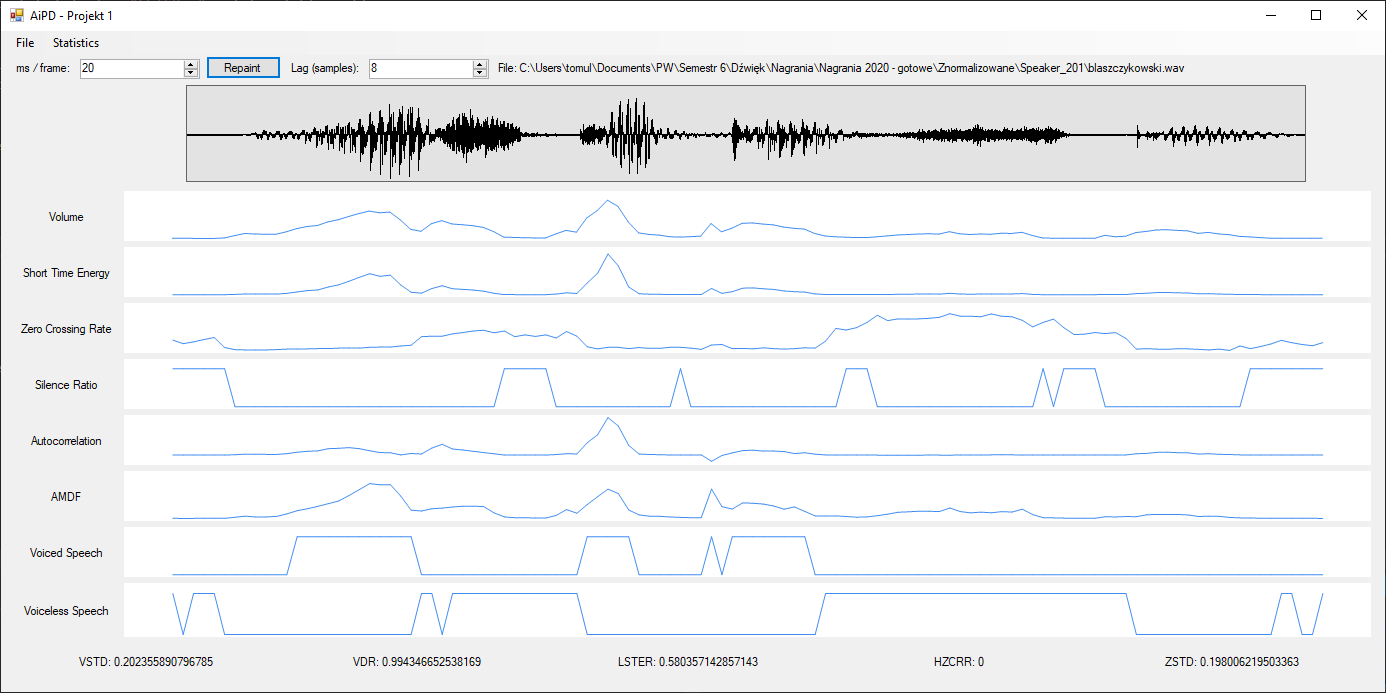
\includegraphics[width=1.0\textwidth]{figures/blaszczykowski_m_20}
\caption{``Błaszczykowski'' - głos męski, 20 ms na ramkę}
\label{fig:blaszczykowski_m_20}
\end{figure}

\begin{figure}[h!]
\centering
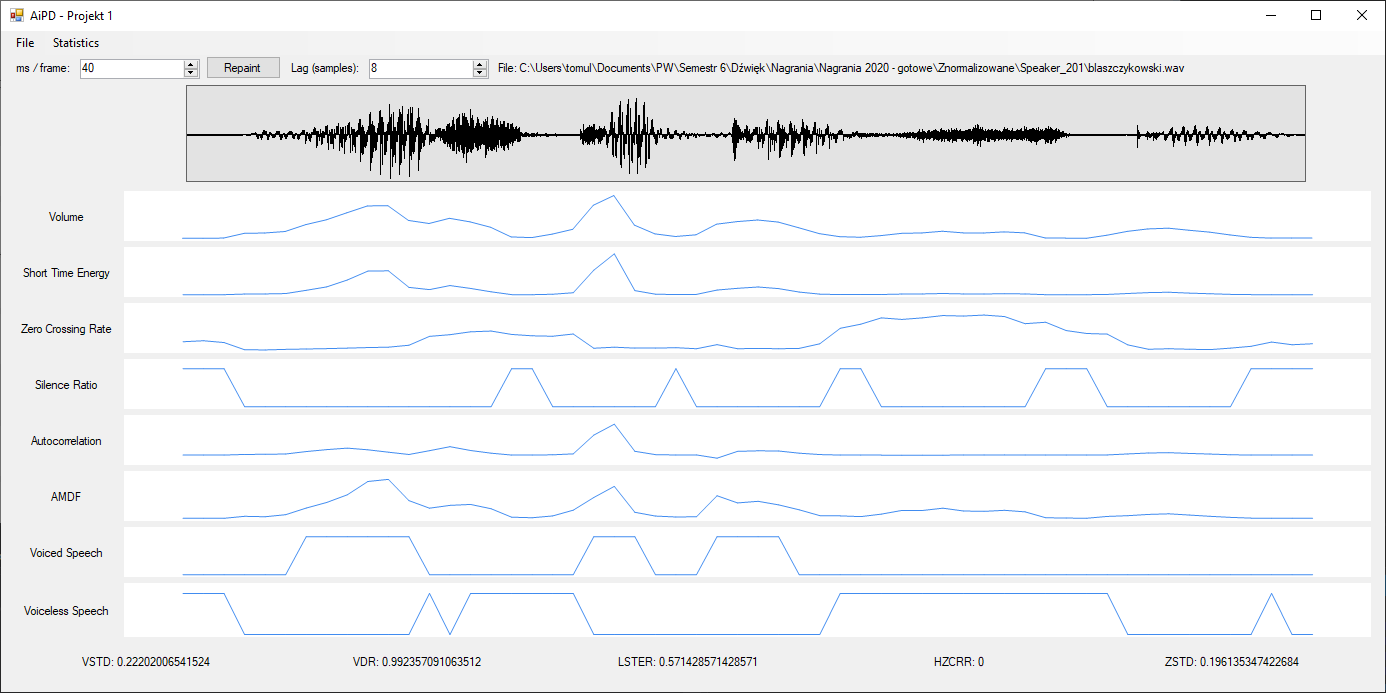
\includegraphics[width=1.0\textwidth]{figures/blasczykowski_m}
\caption{``Błaszczykowski'' - głos męski, 40 ms na ramkę}
\label{fig:blaszczykowski_m}
\end{figure}

W kolejnych przykładach będzie utrzymana stała wartość 40 ms na ramkę.

Rysunek \ref{fig:blaszczykowski_f} przedstawia analizę nagrania damskiego głosu, wypowiadającego
słowo ``Błaszczykowski''. Na tym nagraniu znacznie bardziej uwydatnione są przerwy między sylabami,
co widać na wykresie opisanym ``Silence Ratio''. Widać także, że litera ``y'' obecna w drugiej
sylabie (a więc po pierwszej przerwie) jest wypowiedziana znacznie ciszej. Wpływa to na brak
kwalifikacji tego fragmentu zarówno do mowy dźwięcznej, jak i bezdźwięcznej.

\begin{figure}[h!]
\centering
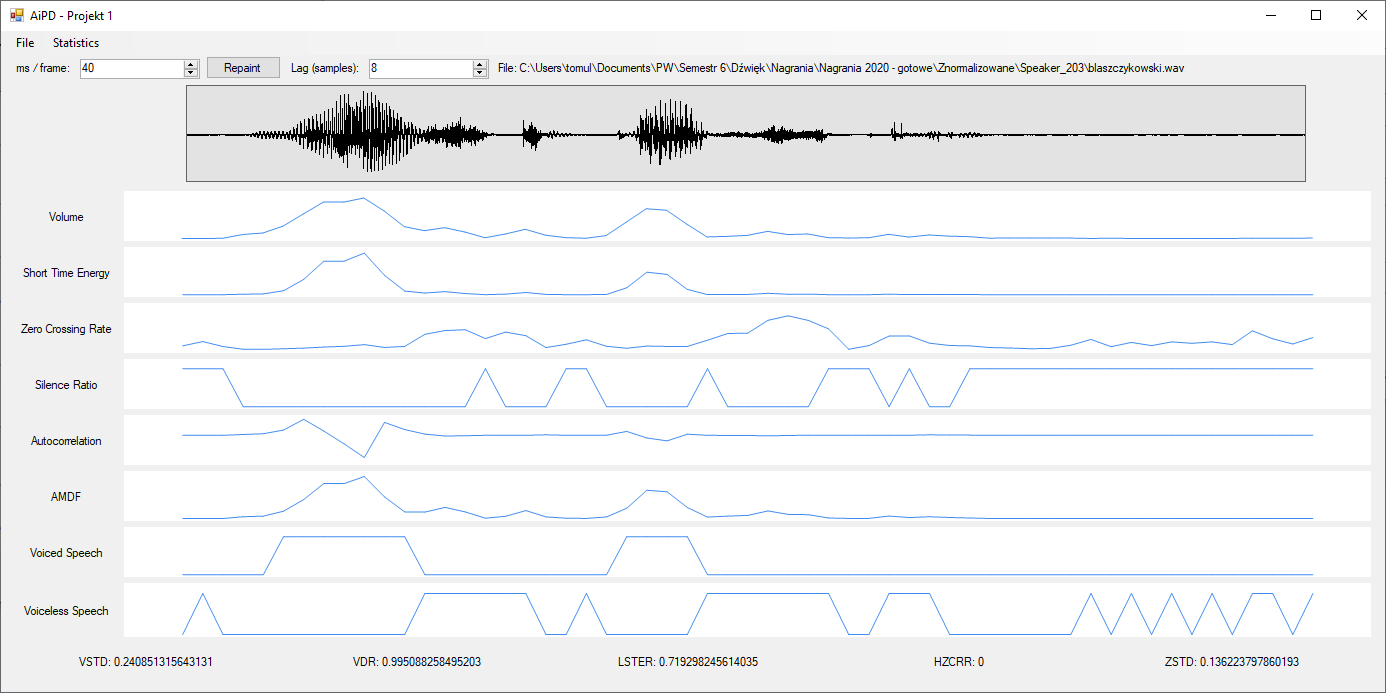
\includegraphics[width=1.0\textwidth]{figures/blasczykowski_f}
\caption{``Błaszczykowski'' - głos żeński}
\label{fig:blaszczykowski_f}
\end{figure}

Na rys. \ref{fig:blaszczykowski_noisy} przedstawiona została analiza nagrania damskiego głosu
wypowiadającego słowo ``Błaszczykowski'' z obecnym słyszalnym hałasem w tle. Hałas, charakteryzujący
się wysokimi wartościami $ZCR$ wpływa bezpośrednio na klasyfikację mowy. Jako mowa dźwięczna
zakwalifikowana jest jedynie pierwsza część pierwszej sylaby. Hałas ten sprawia także, że jako mowa
bezdźwięczna kwalifikowany jest końcowy fragment, uznawany równocześnie za ciszę.

\begin{figure}[h!]
\centering
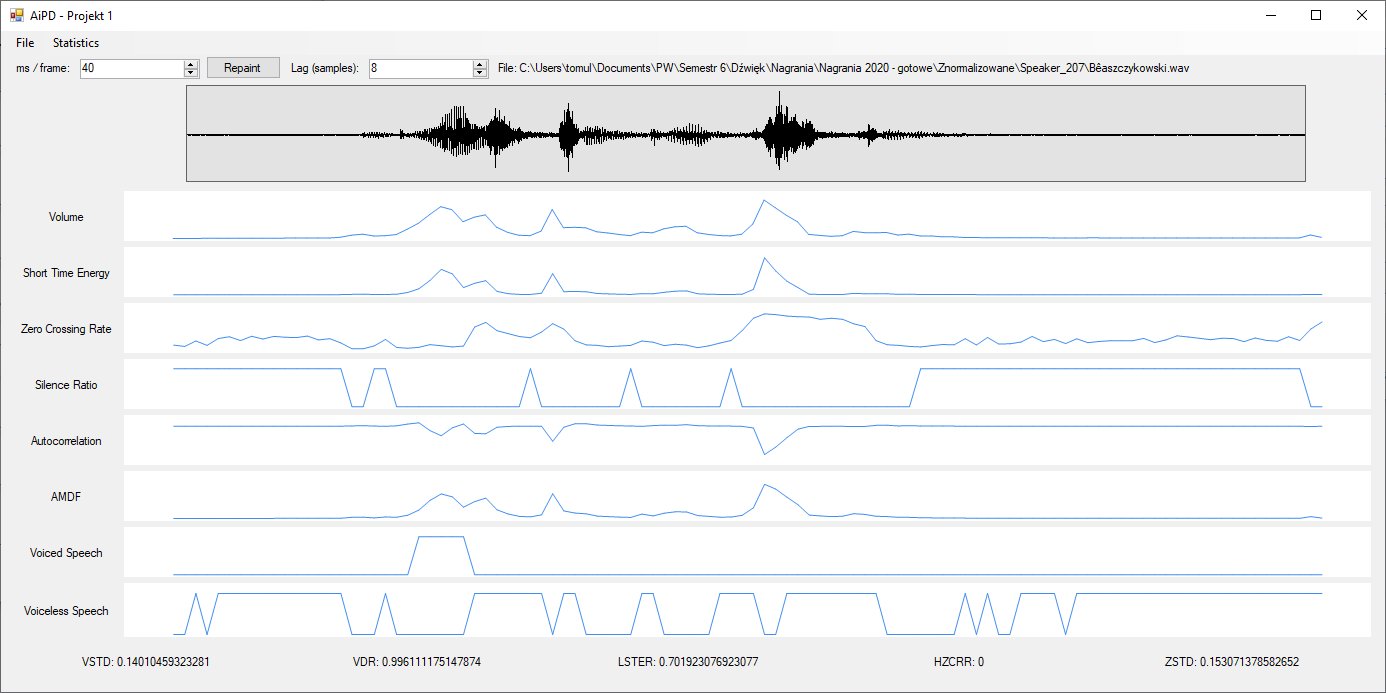
\includegraphics[width=1.0\textwidth]{figures/blasczykowski_noisy}
\caption{``Błaszczykowski'' - hałas w tle}
\label{fig:blaszczykowski_noisy}
\end{figure}

Kolejnym przykładem jest trudne zdanie o rewolwerowcu, wypowiadane przez głos męski. To zdanie
charakteryzuje się jednym wyraźnym bezdźwięcznym ``c''. Doskonale pokazuje to wykres przebiegu
$ZCR$.

\begin{figure}[h!]
\centering
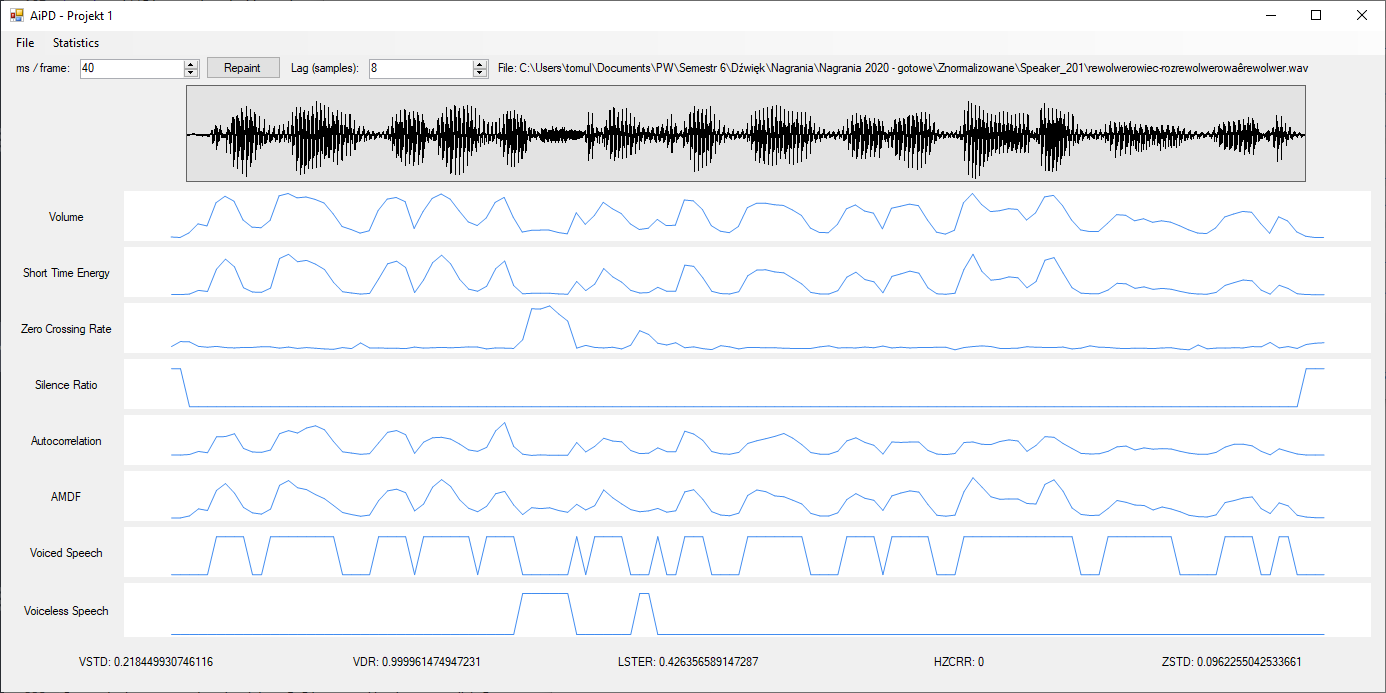
\includegraphics[width=1.0\textwidth]{figures/rewolwerowiec}
\caption{Trudne zdanie o rewolwerowcu - głos męski}
\label{fig:rewolwerowiec}
\end{figure}

Ostatnim wybranym przeze mnie przykładem jest nagranie serii akordów zagranych na syntezatorze
\emph{Roland Juno-60}, a następnie przepuszczonym przez efekt typu delay. Mimo, że wykres energii
wskazuje, że między poszczególnymi akordami jest cisza, w rzeczywistości słyszalny jest tam bardzo
subtelny sygnał generowany przez efekt delay. To nagranie charakteryzuje się także najniższym
współczynnikiem $VSTD$ oraz $LSTER$ ze wszystkich przedstawionych w tej sekcji przykładów.

\begin{figure}[h!]
\centering
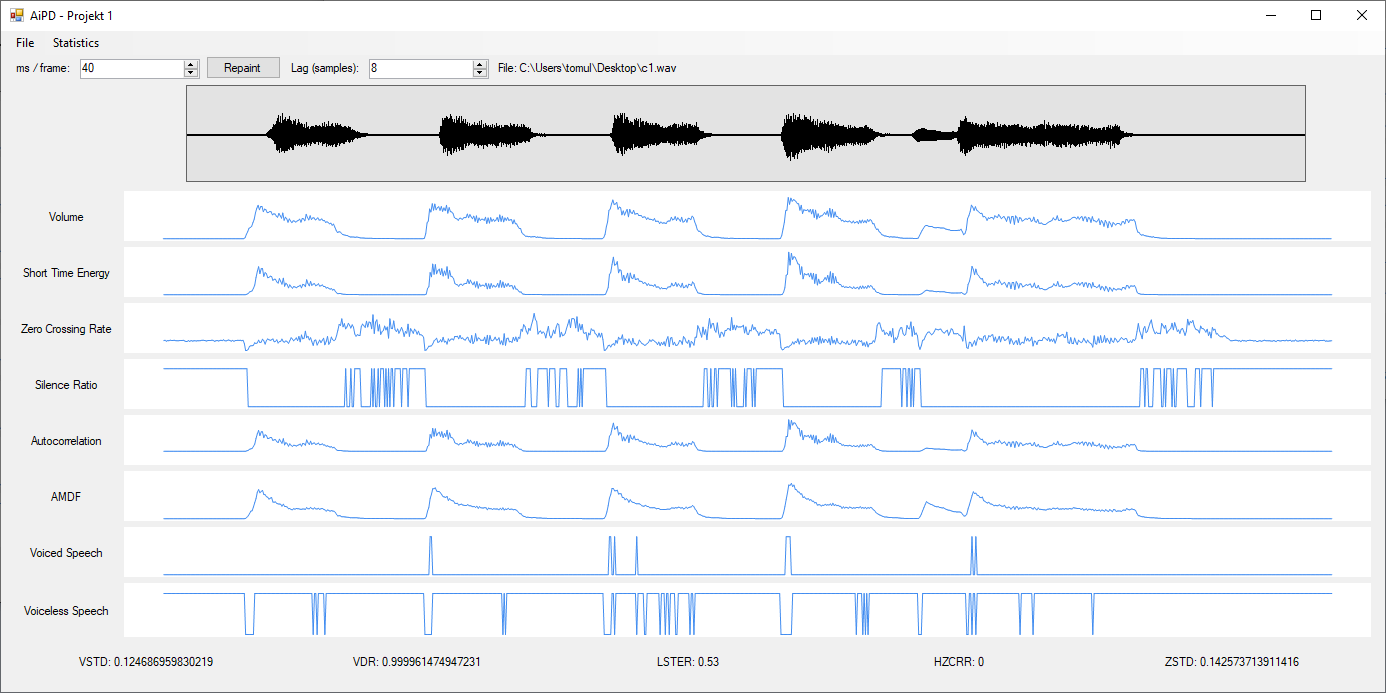
\includegraphics[width=1.0\textwidth]{figures/niemowa}
\caption{Syntezator analogowy}
\label{fig:niemowa}
\end{figure}

\section{Wnioski\label{sec:wnioski}}
Na podstawie wyników i implementacji projektu nasuwają się następujące wnioski:

\subsection{Czy metody zawsze działają dobrze?\label{sec:}}
Przedstawione w tym sprawozdaniu metody działają zadowalająco w stosunku do niskiego nakładu
obliczeń, jakiego wymagają (wszystkie są co najwyżej liniowe względem długości nagrania). Oczywistym
przykładem wskazującym na niepełność metody klasyfikowania mowy jako dźwięcznej lub bezdźwięcznej
jest przykład pokazany na rys. \ref{fig:niemowa}. Można wzbogacić tę metodę o rozróżnianie mowy i
muzyki, jednak nie udało mi się tego zaimplementować.

\subsection{Modyfikacja parametrów\label{sec:modyfikacja_parametrow}}
Metody wykrywania ciszy oraz mowy dźwięcznej i bezdźwięcznej potrzebują w tej implementacji z góry
narzuconych progów dla wartości $ZCR$, $STE$ oraz głośności. Sprawia to, że jeśli progi te nie będą
dobrane dokładnie pod dane nagrania, mogą pojawić się błędy. Bardziej zaawansowane metody rozwiązują
ten problem.

\subsection{Inne wersje metod\label{sec:inne_wersje}}
Prawdopodobnie metoda wykrywania mowy dźwięcznej i bezdźwięcznej wykorzystująca częstotliwość tonu
podstawowego byłaby skuteczniejsza.

\subsection{Napotkane problemy\label{sec:problemy}}
Domyślne wykresy, jakie oferuje biblioteka WinForms okazały się dalekie od oczekiwań jakie można by
mieć w projekcie takim jak ten. Nie udało mi się niestety dostosować ich na tyle, aby czytelne były
zarówno wykresy, jak i wartości je opisujące. W kolejnych projektach planuję wypróbować inne
biblioteki do rysowania wykresów.

Kolejną trudnością, jaką napotkałem i której nie udało mi się rozwiązać, było wczytywanie plików
mp3. Brak płynności w nomenklaturze związanej zarówno z NAudio, jak i formatami plików audio okazał
się dość dużą barierą.

\bibliographystyle{plain}
\bibliography{references}
\end{document}
